\chapter{Physical Layer}\label{sec:osi_physical}
\section{tl;dr}
The first layer of the OSI model is responsible for the physical transmission of data over a medium, with little to no concern for the content involved. It defines the hardware elements used in the communication process, such as cables, switches, and network interface cards (NICs).

\begin{noteblock}
    It might come across as a surprise, but routers are \textbf{not} part of the Physical Layer. The intuition as to why that is is that routers \textit{route}, hence they need to understand the content of the packets they are forwarding. This is a function of the Network Layer (Layer 3) in the OSI model.
\end{noteblock}

The Physical Layer is responsible for:
\begin{itemize}
    \item Converting bits to electrical, optical, or radio signals
    \item Defining voltage levels, timing, and physical data rates
    \item Specifying physical connectors and cable types
    \item Managing the physical topology of the network (which we'll be using Cisco Packet Tracer to visualize)
    \item Synchronizing transmission between devices
\end{itemize}

\newpage

% mediums
\section{Transmission Media}\label{sec:transmission_media}
Different physical media carry the signals that transport our data across networks:

\subsection*{Guided Media}
Guided media confines signals to a specific path (literally "guided" along a cable or fiber). 

\subsubsection*{Twisted Pair Cable}
You probably know this one well, as you find it in most local area networks (LANs) and telephone systems. It consists of pairs of insulated copper wires twisted together to reduce electromagnetic interference.

\begin{figure}[h]
    \centering
    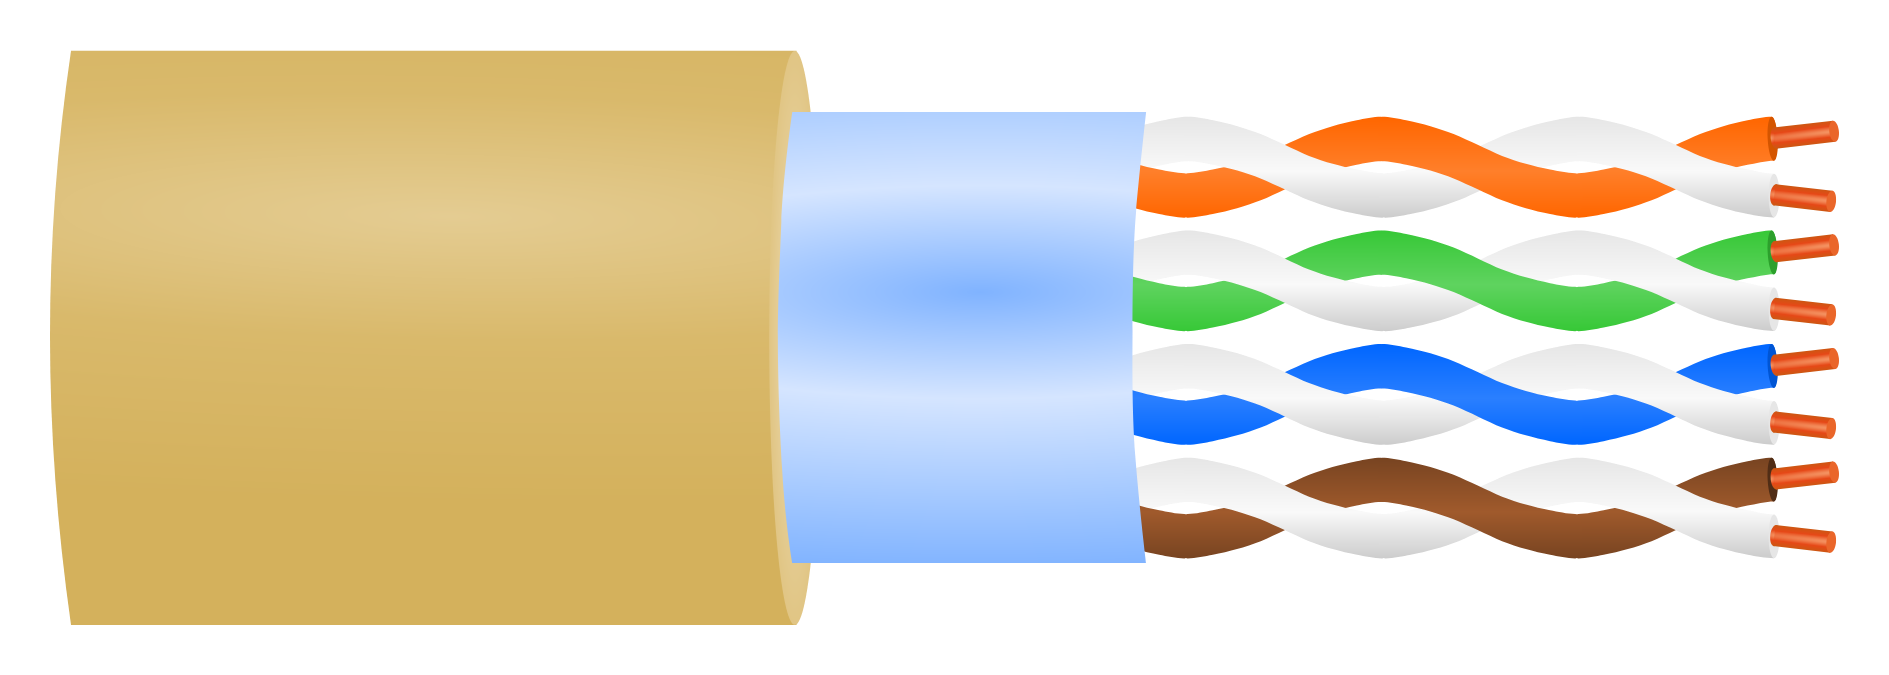
\includegraphics[width=4cm]{assets/osi/physical/f-utp.png}
    \caption{F-UTP}\label{fig:twisted_pair}
\end{figure}

UTP (Unshielded Twisted Pair) is the most common type, but there are also shielded variants like STP (Shielded Twisted Pair) and F/UTP (Foiled Unshielded Twisted Pair).

\vspace{1em}

\subsubsection*{Coaxial Cable}
Usually used in cable television and broadband\footnote{Everything but dial-up.}.

\begin{figure}[h]
    \centering
    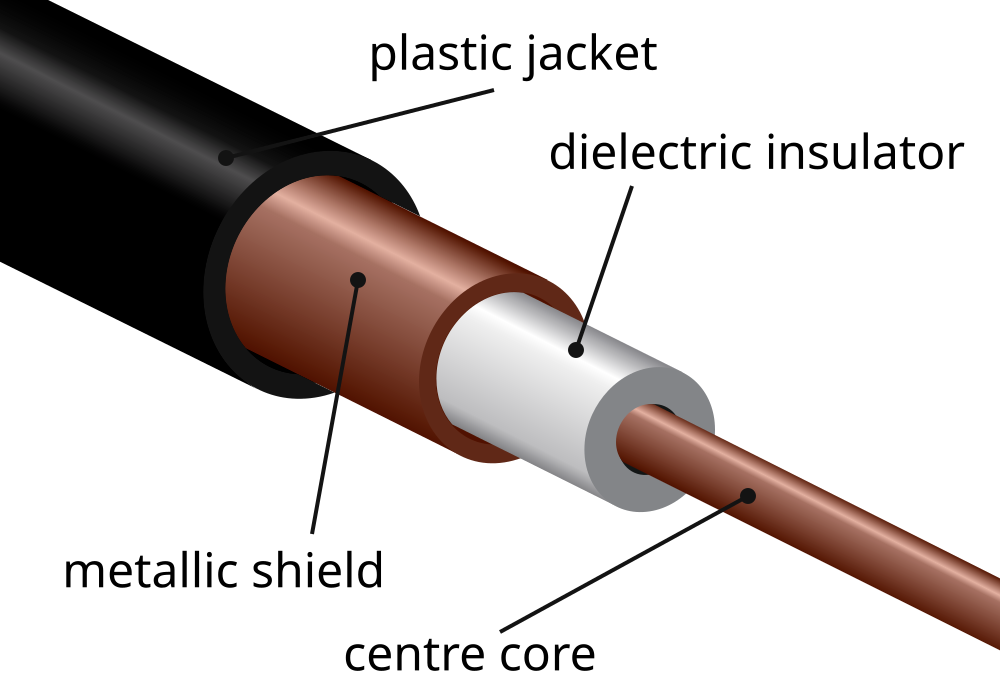
\includegraphics[width=4cm]{assets/osi/physical/coax.png}
    \caption{Coaxial cable structure}\label{fig:coaxial_cable}
\end{figure}

\begin{itemize}
    \item Common in cable TV networks and was used in early Ethernet implementations
    \item Offers better noise immunity than twisted pair with higher bandwidth capacity, which is why radio amateurs still use it
\end{itemize}

\vspace{1em}

\newpage
\subsubsection*{Fiber Optic Cable}
Uses light to transmit data, making it the fastest and most reliable medium available today.

\begin{itemize}
    \item Composed of a core, cladding, and protective outer layer
    \item Immune to electromagnetic interference
    \item Supports high bandwidths
\end{itemize}

\begin{figure}
    \centering
    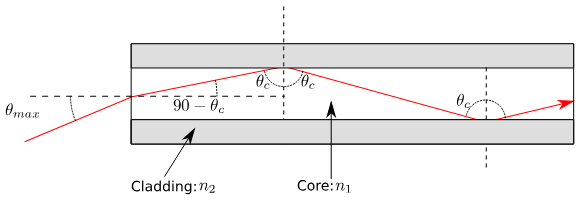
\includegraphics[width=.8\textwidth]{assets/osi/physical/fiber.png}
    \caption{Fiber optic cable structure}\label{fig:fiber_optic}
\end{figure}

\vspace{1em}

\subsection*{Wireless Transmission}
Ever wondered how signals travel through the air? Different types of electromagnetic waves are used for wireless communication, each with its own characteristics.

% assets/osi/physical/spectrum.png
\begin{figure}[h]
    \centering
    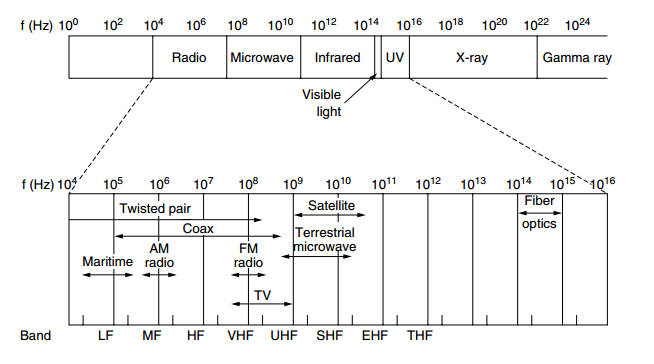
\includegraphics[width=.8\textwidth]{assets/osi/physical/spectrum.png}
    \caption{Electromagnetic spectrum showing different types of waves}\label{fig:em_spectrum}
\end{figure}

\subsubsection*{Radio Waves}
Radio waves are used for various wireless communication systems, including Wi-Fi, Bluetooth, and cellular networks. They can travel long distances (depending on wavelength) and penetrate through obstacles like walls.

\begin{noteblock}
    Fun fact! A lot of appliances like car remotes, thermostats and RC toys operate on the 433 MHz frequency band, which is a part of the radio spectrum. This is a perfect entry point if you'd like to hack your own devices or learn about radio communication.
\end{noteblock}

\subsubsection*{Microwaves}
Contrary to popular belief, microwaves are not just for cooking food. They are also used for point-to-point communication links, satellite communications, and some Wi-Fi networks. Microwaves have shorter wavelengths than radio waves, allowing them to carry more data, but faster attenuation\footnote{
    Attenuation: Reduction in signal strength as it travels through a medium, which can be caused by absorption, scattering, or reflection. 
    This is why we need repeaters/amplifiers!
} over distance.

\section{Standards and Specifications}
\subsection*{Ethernet Standards}
\begin{table}[h]
    \centering
    \begin{tabular}{|c|c|c|c|}
        \hline
        \textbf{Standard} & \textbf{Speed} & \textbf{Media} & \textbf{Distance} \\
        \hline
        10BASE-T & 10 Mbps & Cat3 UTP & 100m \\
        100BASE-TX & 100 Mbps & Cat5 UTP & 100m \\
        1000BASE-T & 1 Gbps & Cat5e UTP & 100m \\
        10GBASE-T & 10 Gbps & Cat6a UTP & 100m \\
        1000BASE-SX & 1 Gbps & Multi-mode fiber & 550m \\
        \hline
    \end{tabular}
    \caption{Common Ethernet Physical Layer Standards}\label{tab:ethernet_standards}
\end{table}

\subsection*{WiFi Standards}
\begin{itemize}
    \item 802.11a: 5 GHz, up to 54 Mbps
    \item 802.11b: 2.4 GHz, up to 11 Mbps
    \item 802.11g: 2.4 GHz, up to 54 Mbps
    \item 802.11n: 2.4/5 GHz, up to 600 Mbps
    \item 802.11ac: 5 GHz, up to 6.9 Gbps
    \item 802.11ax (WiFi 6): 2.4/5 GHz, up to 9.6 Gbps
\end{itemize}

\section{Signal Degradation}
Oh how we wish that signals could travel forever without losing strength! Unfortunately, they don't. As signals travel through a medium, they can degrade due to various factors like noise, interference, and attenuation.

This degradation can lead to errors in data transmission, which is why we need error detection and correction mechanisms in higher layers of the OSI model.

\subsection*{Shannon's Theorem and Channel Capacity}
Claude Shannon's groundbreaking work established the theoretical limits of data transmission over noisy channels. Shannon's theorem states that the maximum data rate (channel capacity) C of a noisy channel is given by:

\begin{equation}
C = B \log_2(1 + SNR)
\end{equation}

Where:
\begin{itemize}
    \item C = Channel capacity in bits per second (bps)
    \item B = Bandwidth in Hz
    \item SNR = Signal-to-Noise Ratio (linear, not in dB)
\end{itemize}

This formula tells us that even in the presence of noise, we can achieve error-free communication as long as our data rate doesn't exceed the channel capacity.

\subsection*{Nyquist's Theorem}
For noiseless channels, Harry Nyquist determined the maximum signaling rate. Nyquist's theorem states that the maximum data rate over a noiseless channel is:

\begin{equation}
C = 2B \log_2(V)
\end{equation}

Where:
\begin{itemize}
    \item C = Maximum data rate in bps
    \item B = Bandwidth in Hz
    \item V = Number of discrete signal levels
\end{itemize}

\begin{importantblock}
    Shannon's theorem considers noise and gives us the theoretical maximum for any channel, while Nyquist's theorem applies only to ideal, noiseless channels. In practice, Shannon's limit is more realistic since all real-world channels have noise.
\end{importantblock}

These theorems show us why we can't simply increase data rates indefinitely (which is something we really like doing when tackling complex problems) - physics imposes hard limits on information transmission!
% modulation
\section{Data Exchange}
Think of it like this: you want to send a message to your friend across the room. You could:
\begin{itemize}
    \item Flash a light on and off (optical)
    \item Tap on the table (mechanical vibrations)
    \item Speak out loud (sound waves)
\end{itemize}

In networks, we do something similar but with electricity, light, or radio waves. We're just changing something physical that the receiver can detect - like voltage going up and down, light getting brighter and dimmer, or radio waves shifting frequency.

\begin{importantblock}
    The process of converting bits into signals is called \textbf{modulation}, and the reverse process is called \textbf{demodulation}.
\end{importantblock}



\subsection{The Reality Check}

Here's where it gets interesting. In an electrical engineer's ideal world, digital signals would look like perfect rectangles - instant jumps from 0 to 1. But physics says that the harsh reality is that a perfect one is impossible to achieve in practice\footnote{Source -- \href{https://en.wikipedia.org/wiki/Square_wave_(waveform)\#Characteristics_of_imperfect_square_waves}{https://en.wikipedia.org/wiki/Square\_wave\_(waveform)}}, due to the lack of infinite bandwidth required to create it. Real signals are always more sinusoidal, with smooth transitions between high and low states.

\begin{figure}[h]
    \centering
    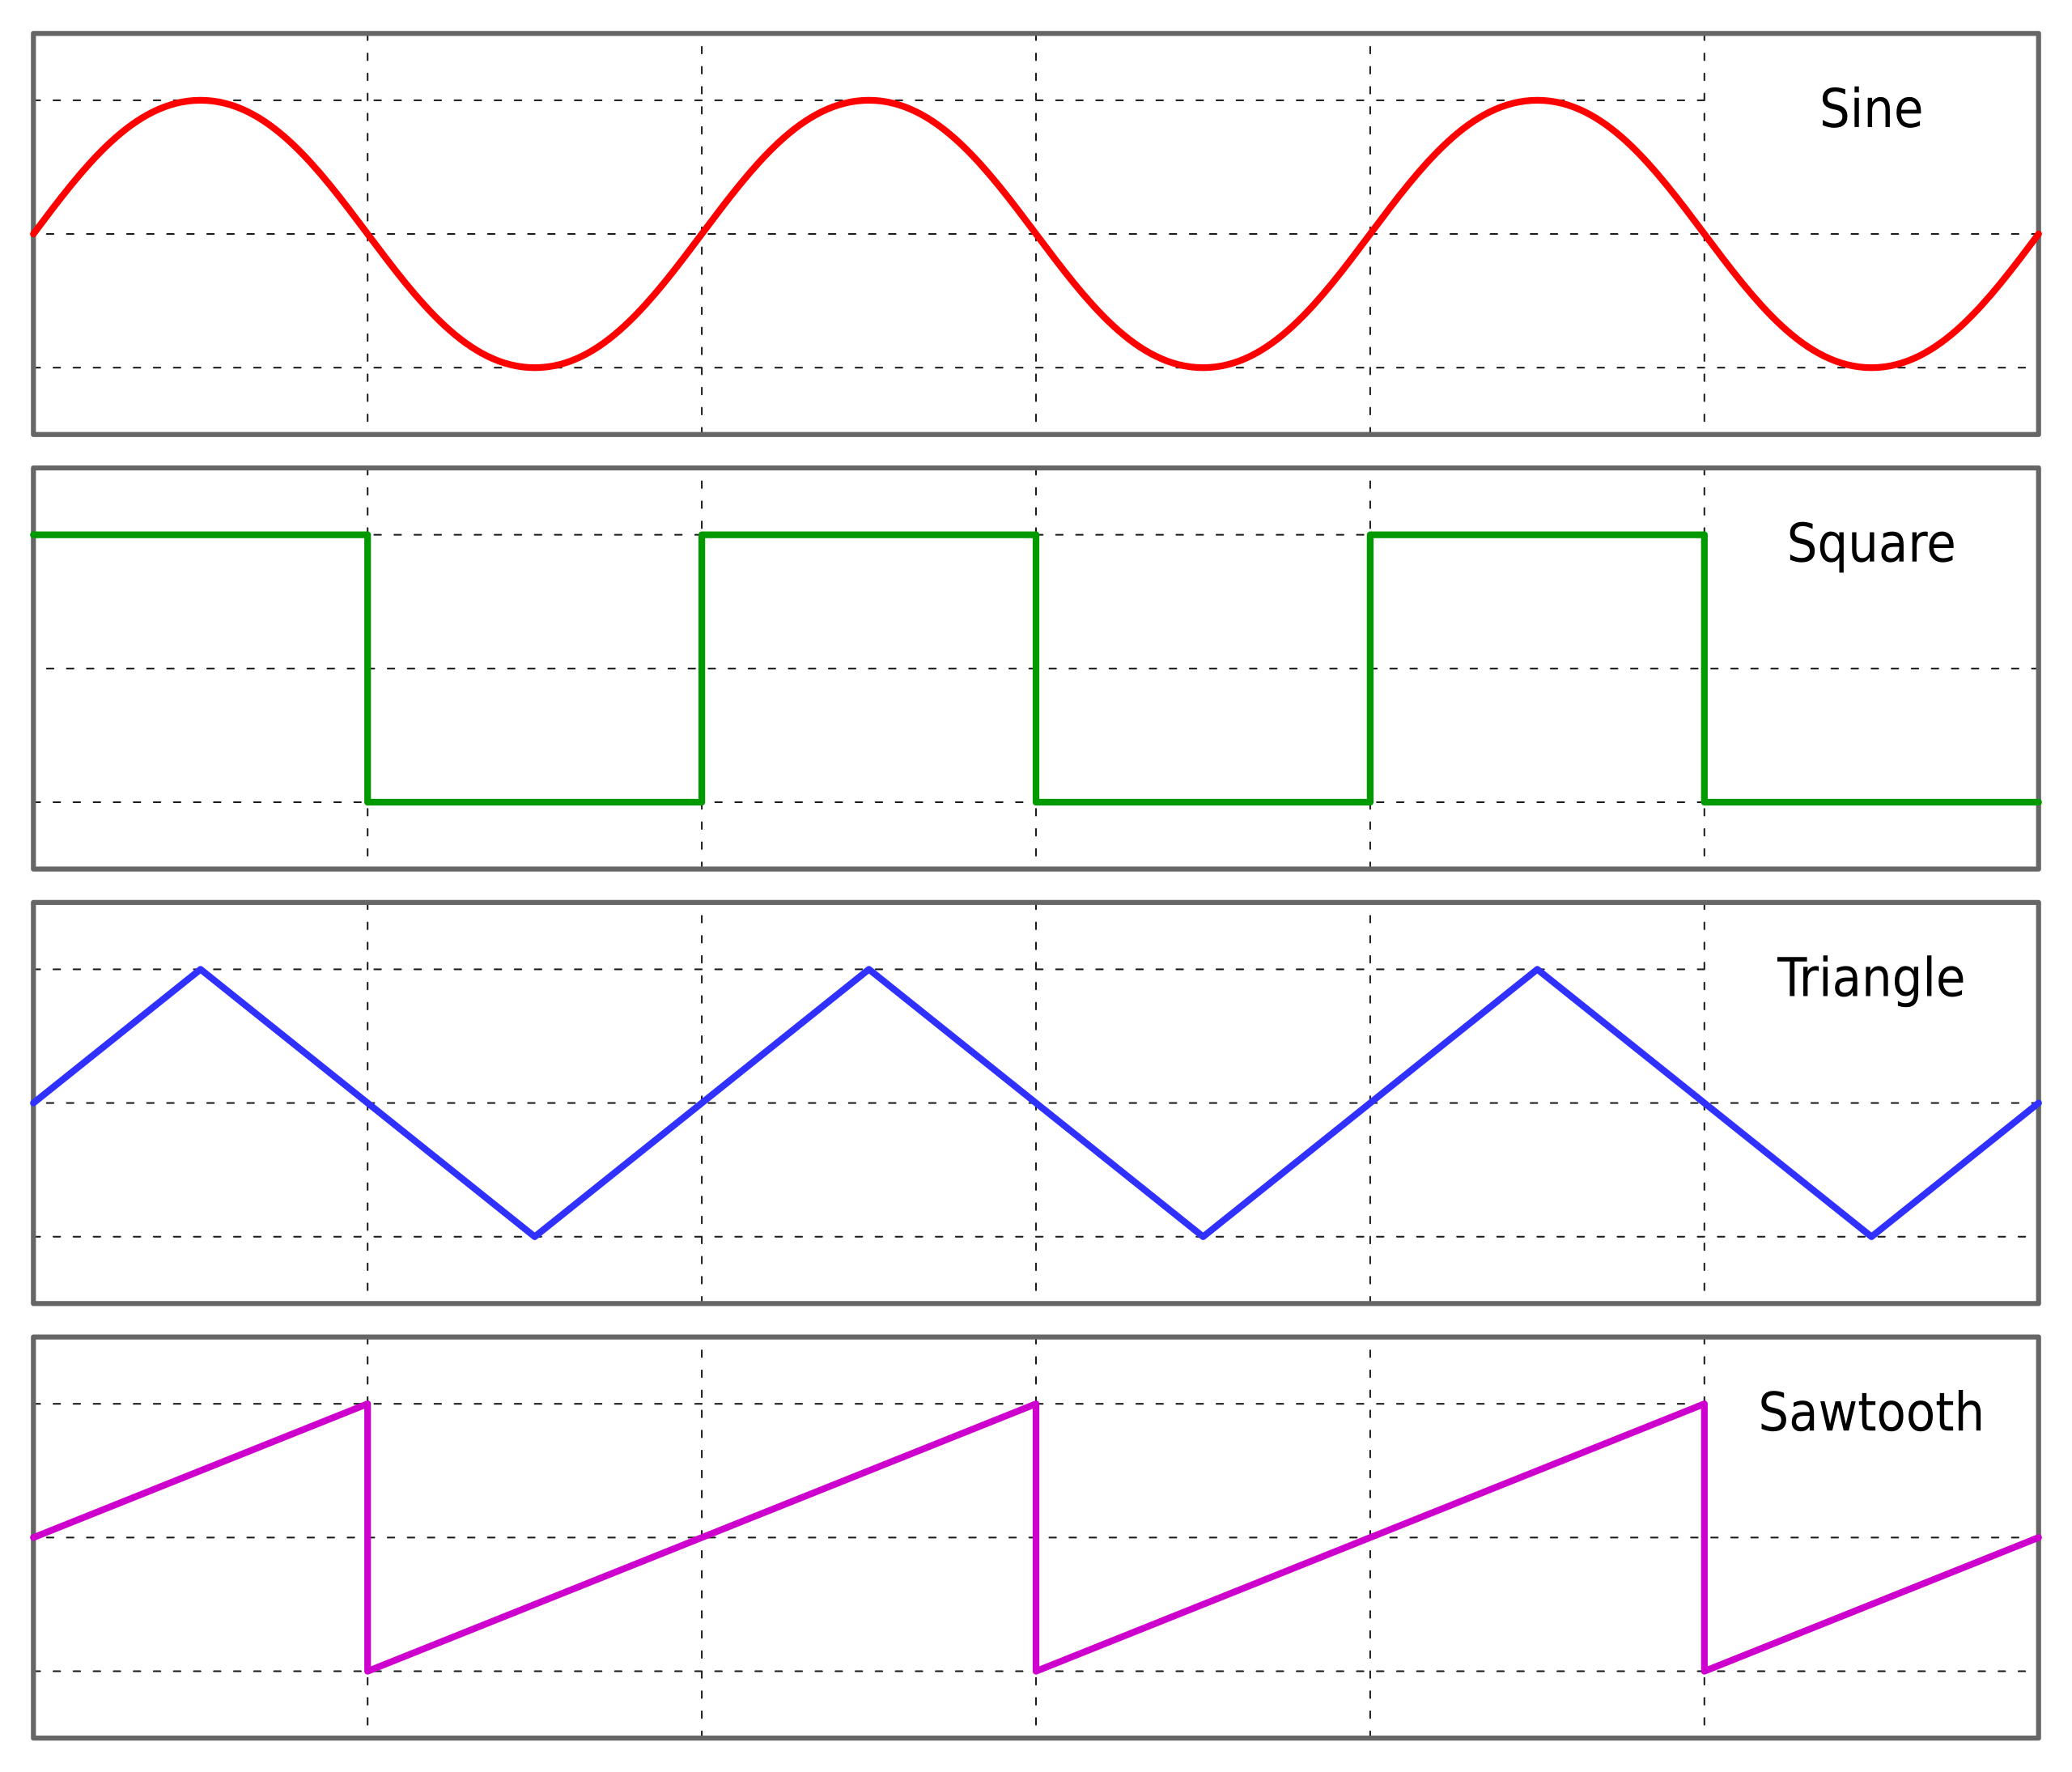
\includegraphics[width=.7\textwidth]{assets/osi/physical/waves.png}
    \caption{Theoretical waves}\label{fig:theoretical_waves}
\end{figure}

In practice, we use analog signals to transmit digital information. They are continuous and can take any value within a range. At the receiver, we need to convert them back to discrete digital values (\texttt{1} or \texttt{0}) through a process called \textbf{sampling and quantization}. The receiver samples the analog signal at specific time intervals and uses threshold levels to determine whether each sample represents a \texttt{1} or \texttt{0}.

Let's look at a simple example of a 1-bit ADC (Analog to Digital Converter) that converts a voltage level into a bit value:

% assets/osi/physical/adc_plot.png
\begin{figure}[h]
    \centering
    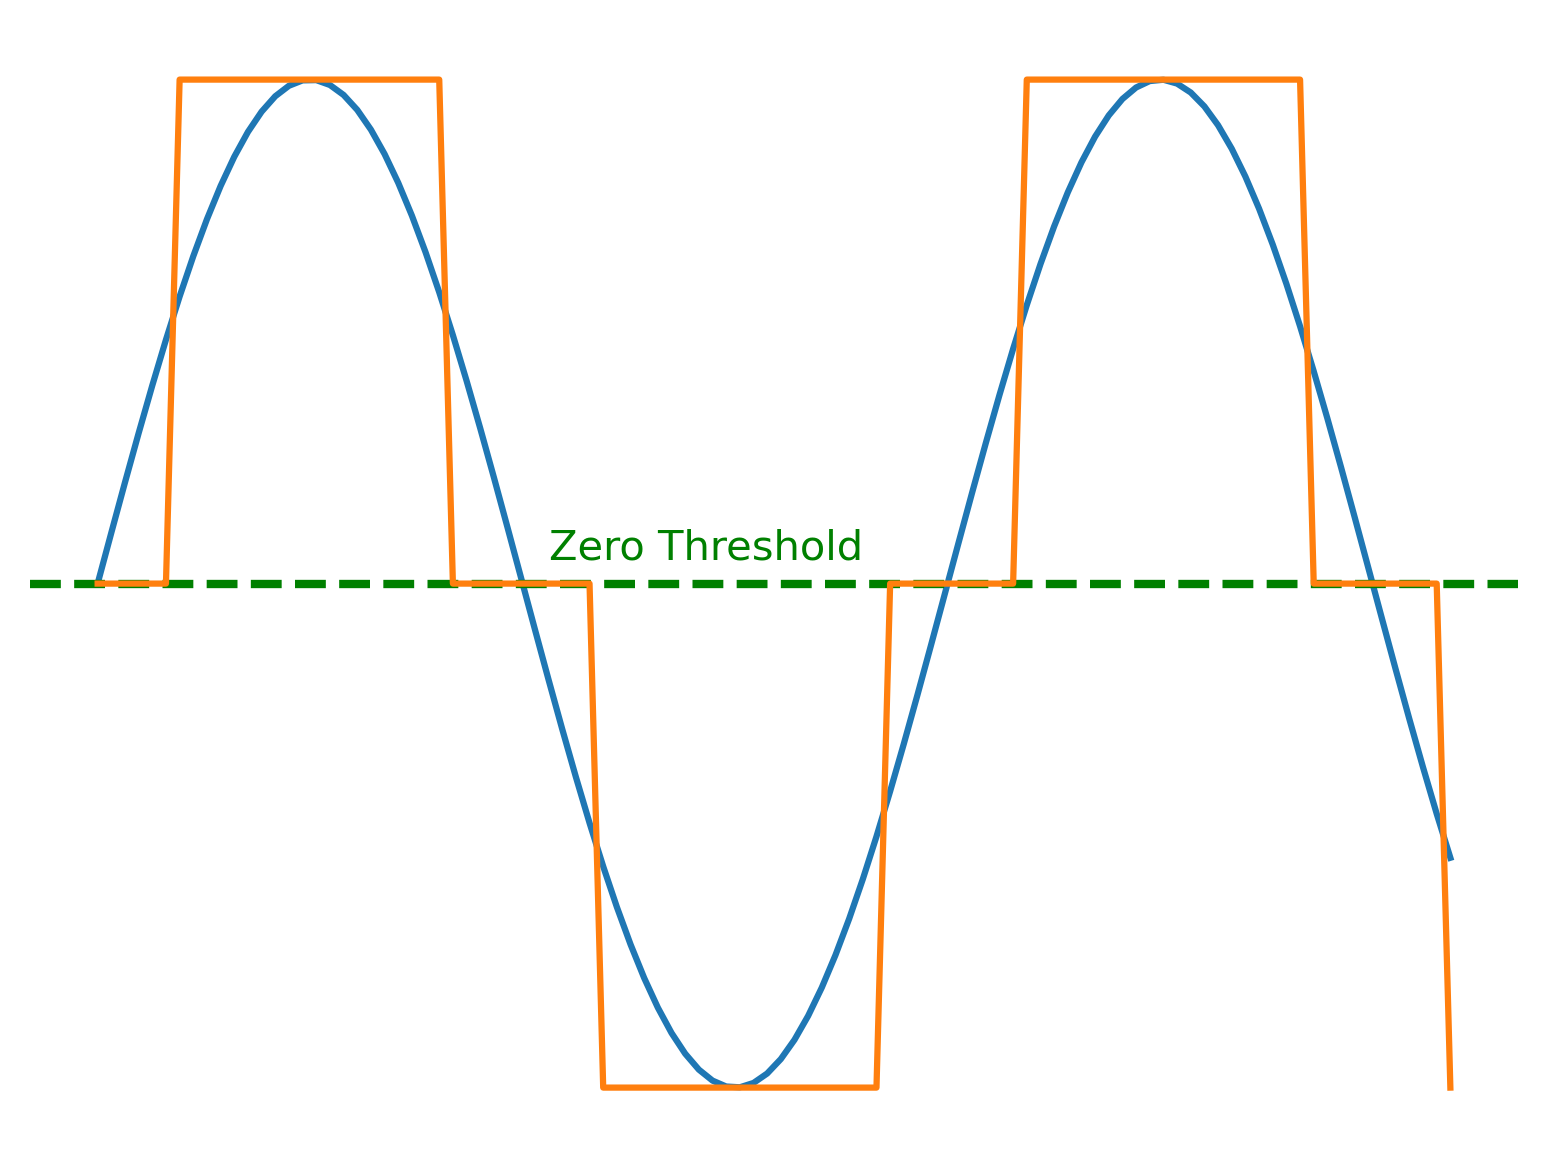
\includegraphics[width=.5\textwidth]{assets/osi/physical/adc_plot.png}
    \caption{Example of a 1-bit ADC converting voltage levels to bits}\label{fig:adc_plot}
\end{figure}

However, as you can probably guess, there are infinite ways for us to interpret this graph. It could correspond to \texttt{1010} or \texttt{1111000011110000} and so on. 
This is where clock signals come into play, which help us determine when to sample the signal and how to interpret it.

\subsection*{Let's talk timing $\star$}
Clocks or timing signals are present in all hardware communication. 

The idea is to ensure that both sender and receiver are synchronized in their understanding of when bits are being sent and received. 


There are two main types of synchronization:
\begin{itemize}
    \item Both sender and receiver share a common clock signal (Figure~\ref{fig:clock_sync}) - Synchronous 
    \item Sender and receiver do not share a common clock, but use start and stop bits to indicate the beginning and end of a data frame - Asynchronous
\end{itemize}

\begin{figure}[h]
    \centering
    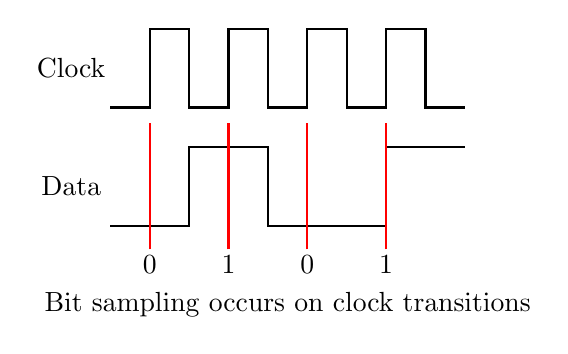
\begin{tikzpicture}
        % Clock signal
        \draw[thick] (0,2) -- (0.5,2) -- (0.5,3) -- (1,3) -- (1,2) -- (1.5,2) -- (1.5,3) -- (2,3) -- (2,2) -- (2.5,2) -- (2.5,3) -- (3,3) -- (3,2) -- (3.5,2) -- (3.5,3) -- (4,3) -- (4,2) -- (4.5,2);
        \node at (-0.5,2.5) {Clock};
        
        % Data signal
        \draw[thick] (0,0.5) -- (1,0.5) -- (1,1.5) -- (2,1.5) -- (2,0.5) -- (3.5,0.5) -- (3.5,1.5) -- (4.5,1.5);
        \node at (-0.5,1) {Data};
        
        % Sampling points
        \foreach \x in {0.5,1.5,2.5,3.5}
            \draw[red,thick] (\x,0.2) -- (\x,1.8);
        
        % Bit values
        \node at (0.5,0) {0};
        \node at (1.5,0) {1};
        \node at (2.5,0) {0};
        \node at (3.5,0) {1};
        
        % Labels
        \node at (2.25,-0.5) {Bit sampling occurs on clock transitions};
    \end{tikzpicture}
    \caption{Example rising edge clock synchronization}\label{fig:clock_sync}
\end{figure}

\vfill
In asynchronous serial\footnote{
    Serial - \textit{one after another} - communication, data is sent one bit at a time over a single channel. This is in contrast to parallel communication. More on that in the Operating Systems course.
} communication, data is organized into discrete blocks called code words of fixed length - usually bytes or ASCII characters (\texttt{char}s are $2^8 = 256$ bits, i.e. a byte). Each code word is framed by:

\begin{figure}[h]
    \centering
    \input{assets/diagrams/physical.latex}
    \caption{Async serial frame structure}\label{fig:async_frame}
\end{figure}

This approach, specifically in the form that we refer to in the figure, is \textbf{character-oriented}.
\vfill
\section{Modulation and Encoding}\label{sec:modulation}
As mentioned earlier, modulation is the process of converting digital data into analog signals for transmission over a physical medium.

\begin{figure}[h]
    \centering
    
\includegraphics[width=\textwidth]{assets/osi/physical/signals/modulation.png}
    \caption{Modulation techniques}\label{fig:modulation_techniques}
\end{figure}

\subsection{The basics}
We'll start with something most people are familiar with, as it is used in consumer radios! The ones you listen to in your car or at home.

Amplitude Modulation (AM) and Frequency Modulation (FM) are two very common modulations used in radio broadcasting, where we are used to hearing music and news. We are used to tuning our radios to a specific frequency ($\approx$ 80-100 MHz for FM and usually way lower for AM) to listen to our favorite stations.

There's also Phase Modulation (PM), where the phase of the carrier wave is varied according to the input signal.
\begin{figure}[h]
    \centering
    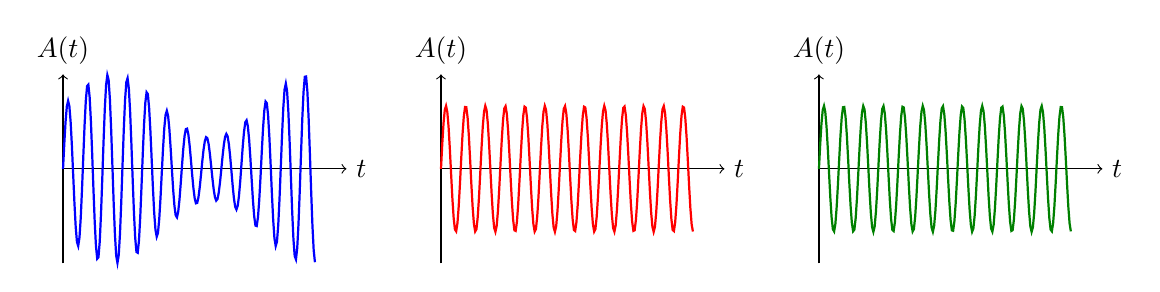
\begin{tikzpicture}[scale=0.8]
        % AM Signal
        \begin{scope}[shift={(0,0)}]
            \draw[->] (0,0) -- (4.5,0) node[right] {$t$};
            \draw[->] (0,-1.5) -- (0,1.5) node[above] {$A(t)$};
            \draw[domain=0:4,samples=200,thick,blue] plot (\x,{(1+0.5*sin(2*\x r))*sin(20*\x r)});
        \end{scope}
        
        % FM Signal
        \begin{scope}[shift={(6,0)}]
            \draw[->] (0,0) -- (4.5,0) node[right] {$t$};
            \draw[->] (0,-1.5) -- (0,1.5) node[above] {$A(t)$};
            \draw[domain=0:4,samples=200,thick,red] plot (\x,{sin(20*\x r + 2*sin(2*\x r))});
        \end{scope}
        
        % PM Signal
        \begin{scope}[shift={(12,0)}]
            \draw[->] (0,0) -- (4.5,0) node[right] {$t$};
            \draw[->] (0,-1.5) -- (0,1.5) node[above] {$A(t)$};
            \draw[domain=0:4,samples=200,thick,green!50!black] plot (\x,{sin(20*\x r + 0.5*sin(2*\x r))});
        \end{scope}
    \end{tikzpicture}
    \caption{Graphical representation of \textcolor{blue}{AM}, \textcolor{red}{FM}, and \textcolor{green!50!black}{PM} signals.}\label{fig:modulation_math}
\end{figure}


But wait, we have only heard voices and music, not bits! How does that work?

The answer lies in \textbf{digital modulation}! While AM and FM were originally designed for analog voice transmission, the same radio frequencies can carry digital data using techniques like DMR, WSPR, and many, many more.
These digital protocols use discrete changes in amplitude, frequency, or phase to represent bits.

For example, in WSPR, a \texttt{1} might be represented by a short burst of a specific frequency, while a \texttt{0} might be represented by silence or a different frequency - this is called \textbf{frequency-shift keying (FSK)}.


\begin{figure}[h]
    \centering
    \begin{subfigure}[b]{0.2\textwidth}
        \centering
        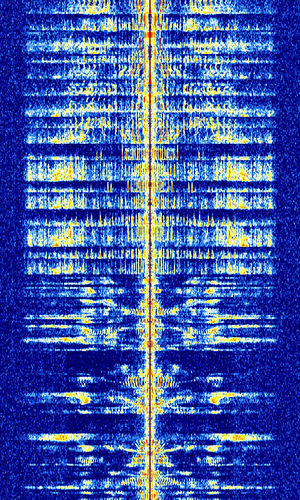
\includegraphics[width=\textwidth]{assets/osi/physical/signals/am_voice.png}
        \caption{AM Voice Signal}
        \label{fig:am_voice}
    \end{subfigure}
    \hspace{1em}
    \begin{subfigure}[b]{0.2\textwidth}
        \centering
        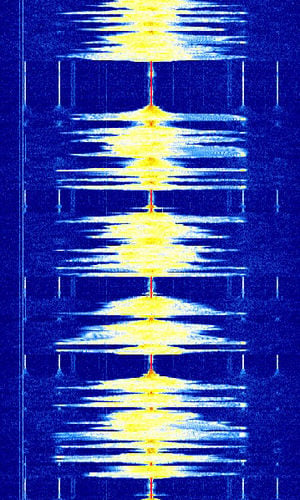
\includegraphics[width=\textwidth]{assets/osi/physical/signals/fm_voice.png}
        \caption{FM Voice Signal}
        \label{fig:fm_voice}
    \end{subfigure}
    \hspace{1em}
    \begin{subfigure}[b]{0.2\textwidth}
        \centering
        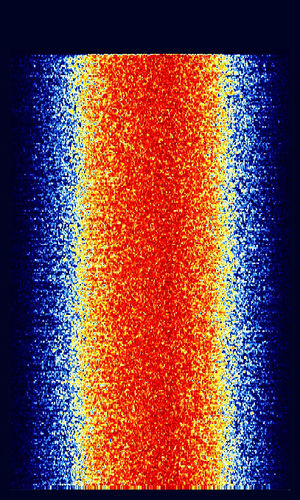
\includegraphics[width=\textwidth]{assets/osi/physical/signals/dmr.png}
        \caption{DMR Digital Signal}
        \label{fig:dmr_digital}
    \end{subfigure}
    \hspace{1em}
    \begin{subfigure}[b]{0.2\textwidth}
        \centering
        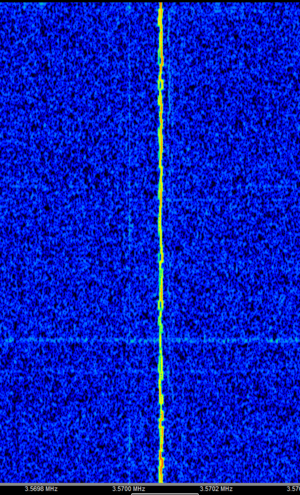
\includegraphics[width=\textwidth]{assets/osi/physical/signals/wspr.png}
        \caption{WSPR Digital Protocol}
        \label{fig:wspr_digital}
    \end{subfigure}
    
    \caption{Comparison of analog voice signals (a, b) vs digital signals (c, d) in the radio spectrum. Sourced from sigidwiki.com}
    \label{fig:analog_vs_digital_signals}
\end{figure}

\newpage
For digital data, modulation becomes synonymous with \textbf{keying}, where we use changes in the signal to represent bits.

\begin{itemize}
    \item Amplitude Shift Keying (ASK) -  A higher amplitude might represent a \texttt{1}, while a lower amplitude represents a \texttt{0}.
    \item Frequency Shift Keying (FSK) - Different frequencies represent different bits.
    \item Phase Shift Keying (PSK) - A phase shift might represent a \texttt{1}, while no shift represents a \texttt{0}.
\end{itemize}
\begin{figure}[h]
    \centering
    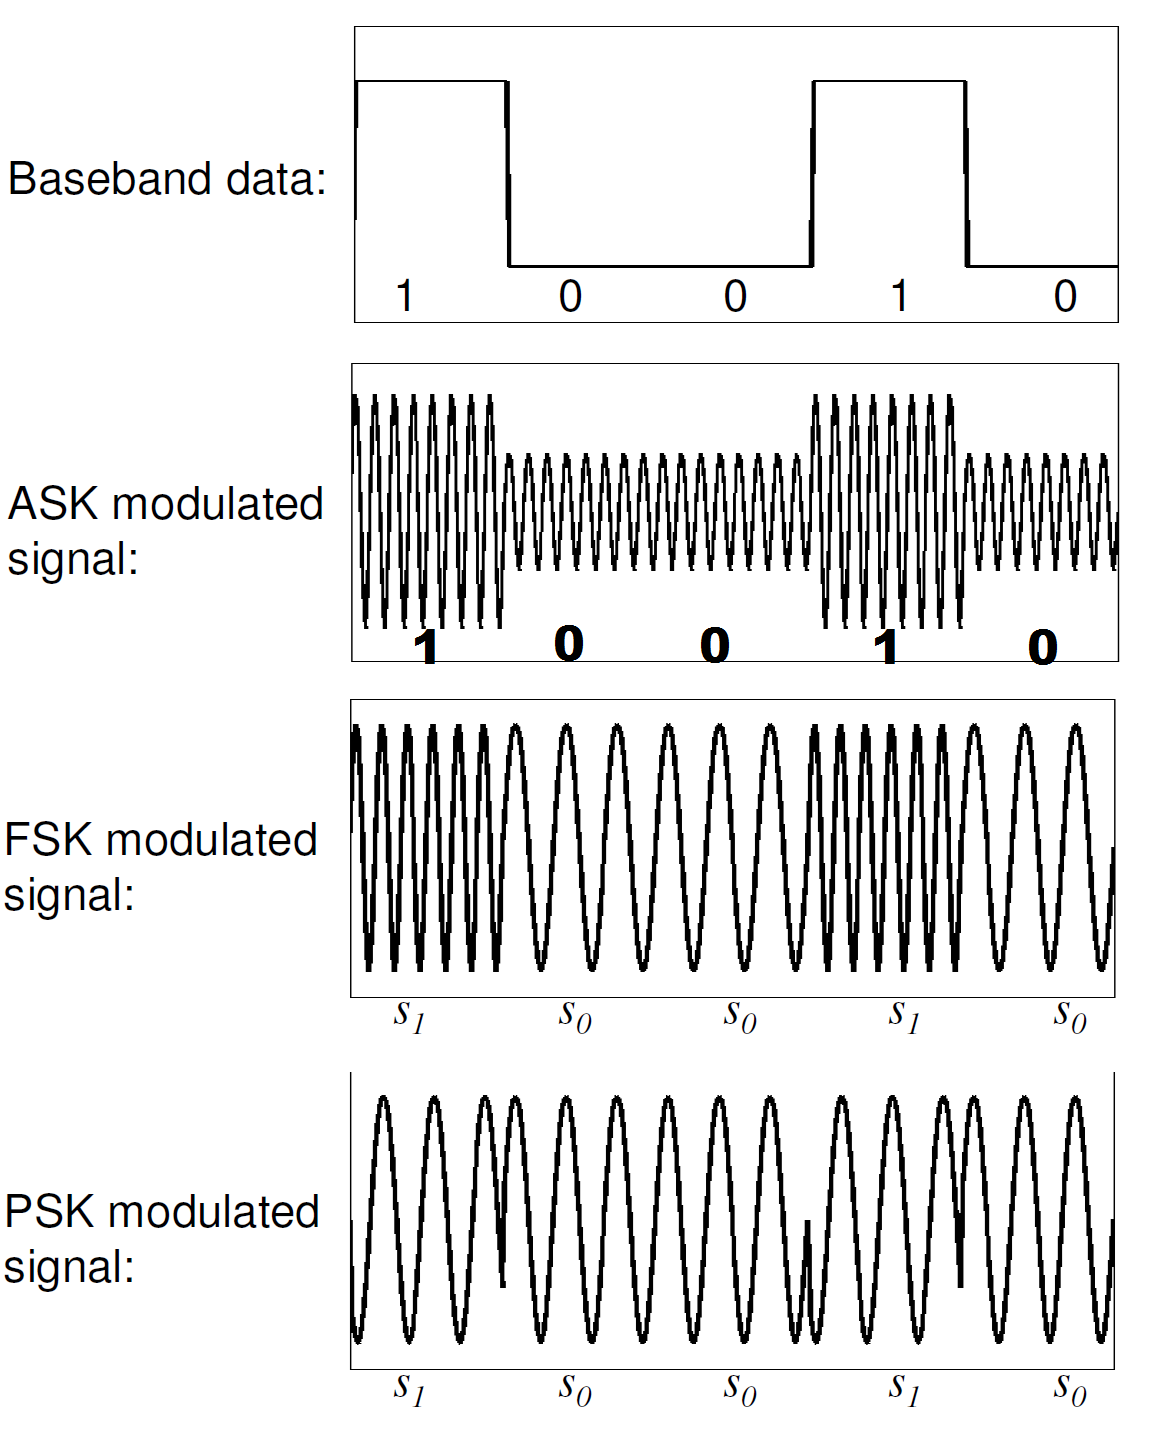
\includegraphics[width=0.45\textwidth]{assets/osi/physical/signals/sk.png}
    \caption{Keying techniques: ASK, FSK, PSK}\label{fig:keying_techniques}
\end{figure}

\subsection{Quadrature Amplitude Modulation (QAM)}
What if we could send multiple bits at once? That's where QAM comes in, which is a combination of both amplitude and phase modulation.

`Quadrature' just means we're using two waves that are perfectly out of sync - 90 degrees out of phase, to be exact (quad = four, so in a circle $\frac{360}{4} = 90$).

\subsubsection{Complex Numbers and QAM $\star$}
To completely understand QAM, we will need to quickly refresh our knowledge of complex numbers. If you are not familiar with them, I recommend reading the \href{https://en.wikipedia.org/wiki/Complex_number}{Wikipedia article}. 

QAM transmits data using two independent carrier waves at the same frequency but shifted 90 degrees apart in phase - called `in-phase' ($I$) and `quadrature' ($Q$) components. This orthogonal\footnote{
    Remember orthogonality! It's a cheat code in signal processing! It means the two signals don't interfere with each other and can be separated at the receiver.
} relationship means the two signals don't interfere with each other and can be separated at the receiver.

Complex numbers provide an elegant mathematical framework for this because:
\begin{itemize}
    \item The real part represents the in-phase ($I$) component
    \item The imaginary part represents the quadrature ($Q$) component  
    \item A 90-degree phase shift is equivalent to multiplication by $i$ (since $e^{i\pi/2} = i$)
    \item Both amplitude and phase information are present in a single complex number $z = $I$ + iQ$
\end{itemize}

\begin{figure}[h]
    \centering
    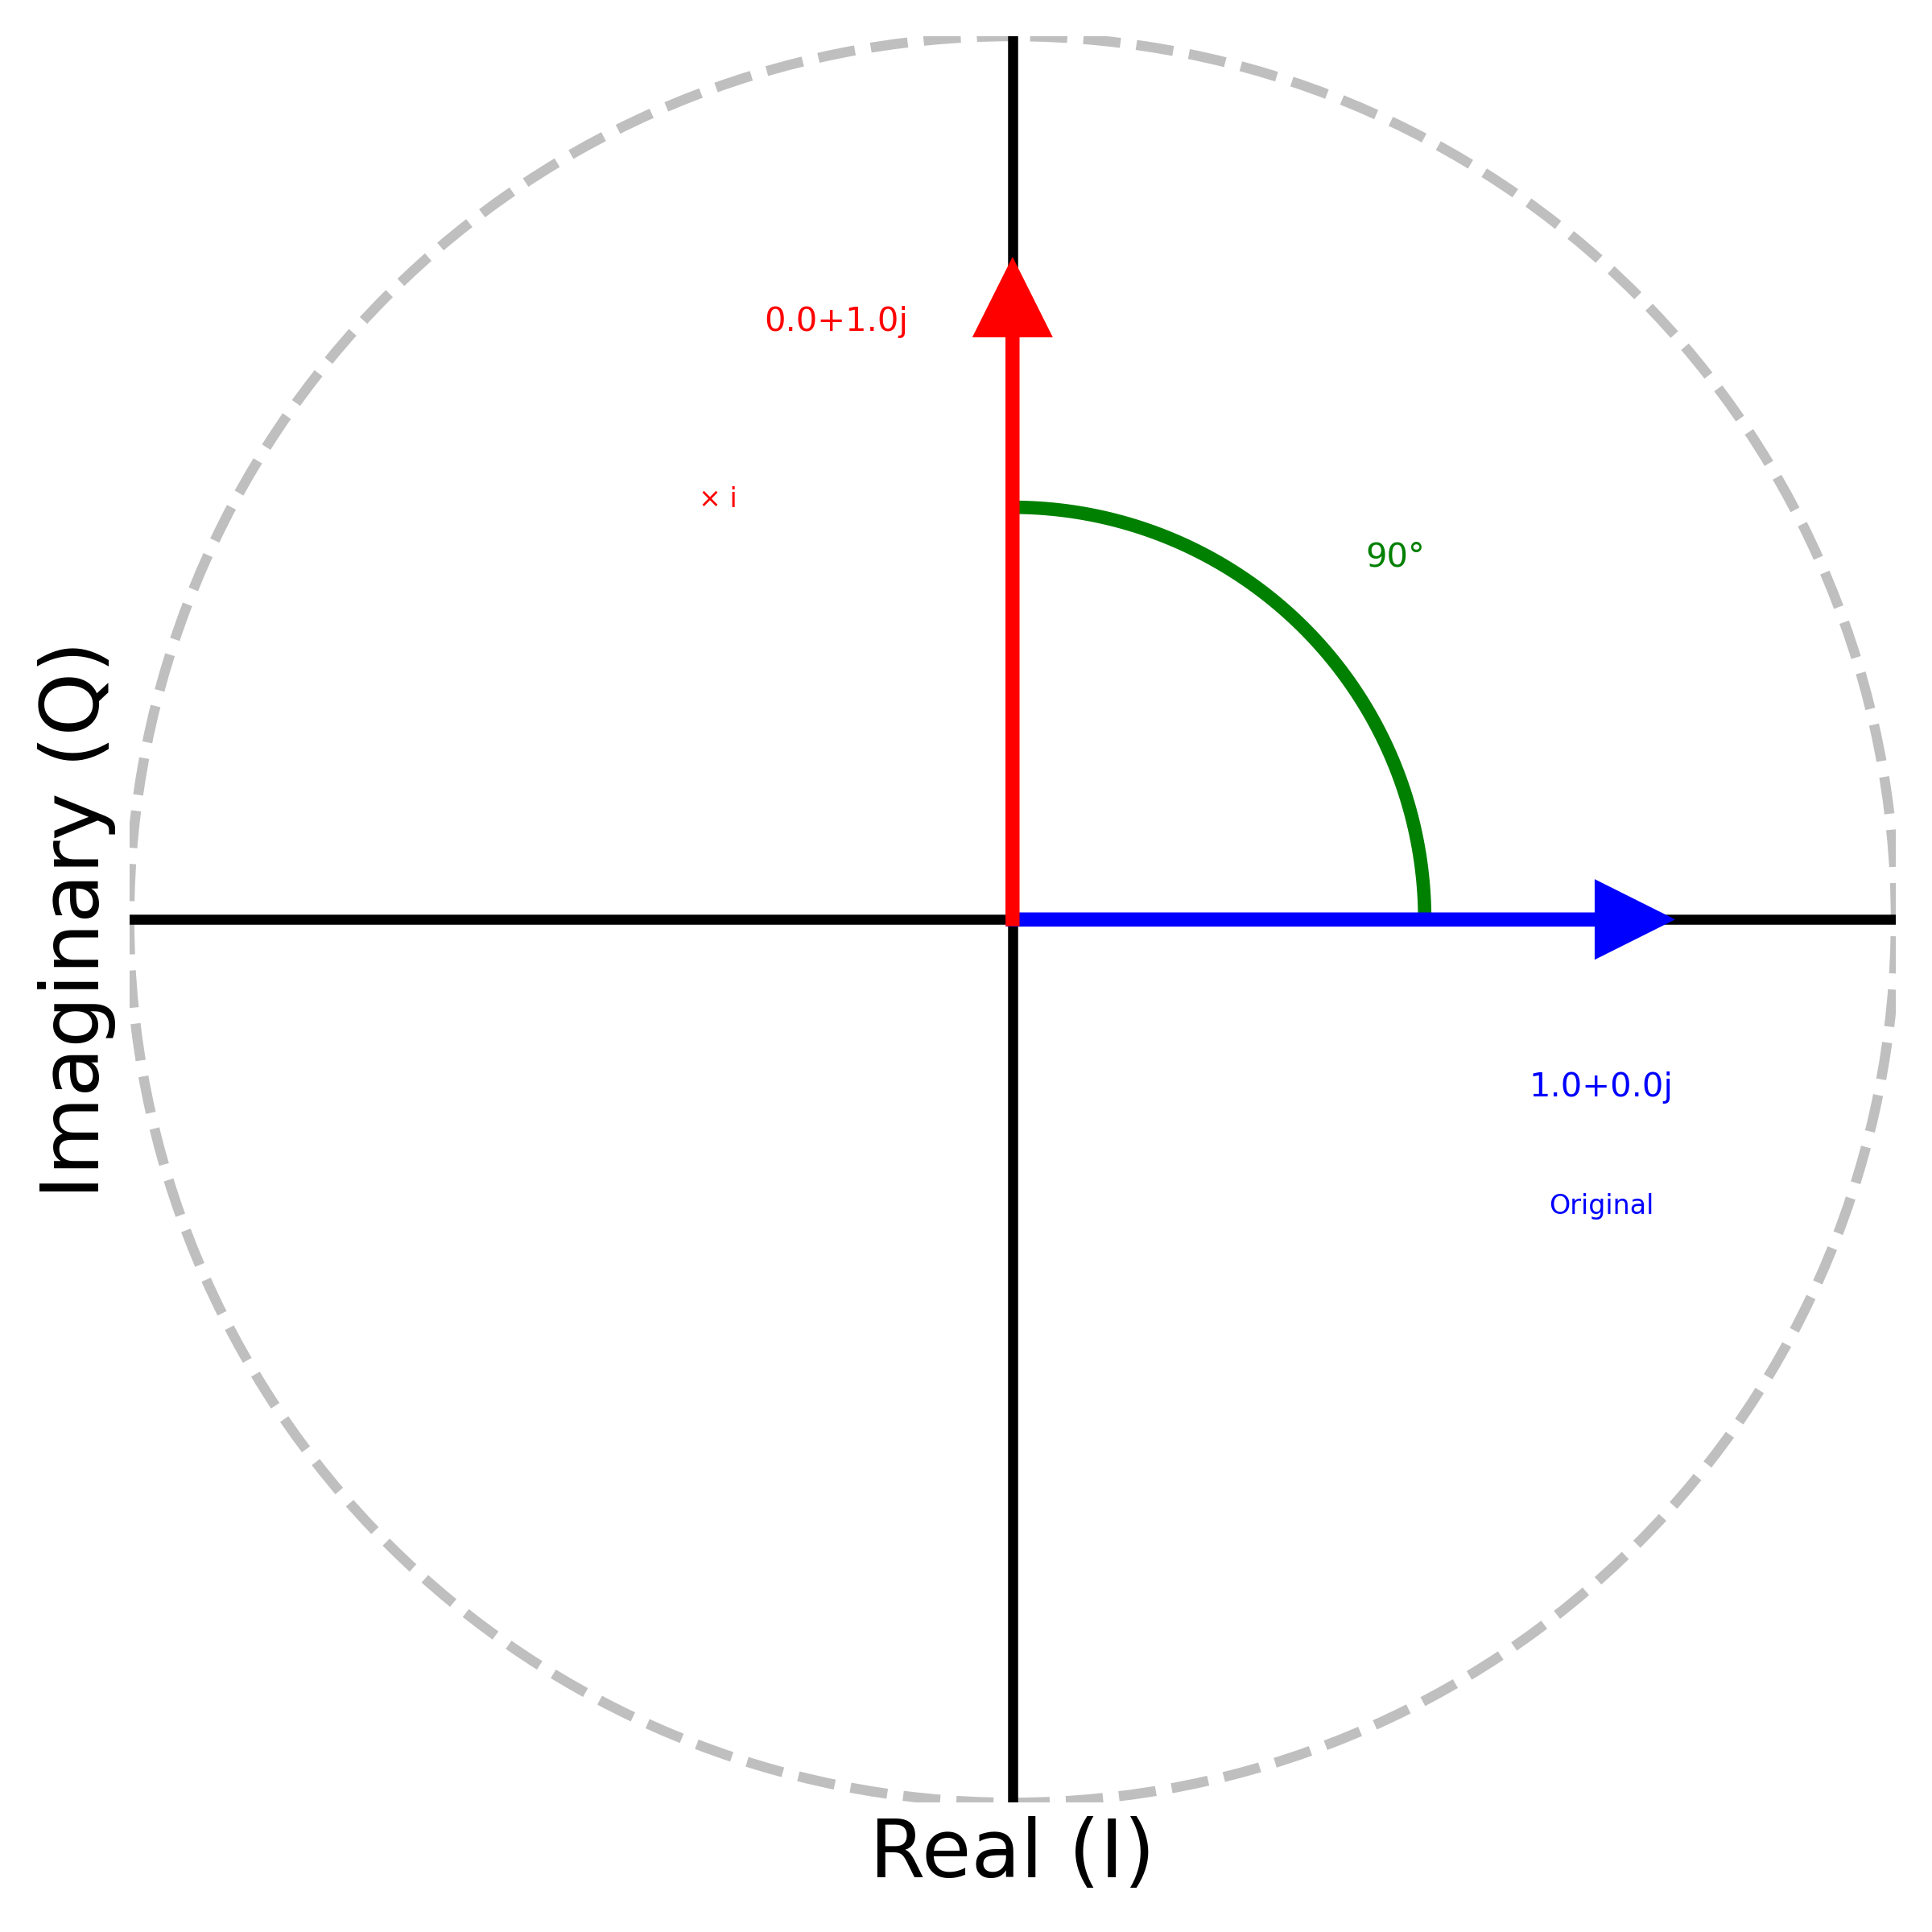
\includegraphics[width=0.5\textwidth]{assets/diagrams/iq.png}
\end{figure}

This is why we call it "Quadrature" - it literally refers to the four quadrants of this complex plane, where signals can point in any direction to encode different bit combinations.

\subsubsection{What does the number mean?}
When working with QAM, we will often see terms like 16-QAM, 64-QAM, etc. These numbers refer to the number of distinct symbols that can be transmitted. For example:
\begin{itemize}
    \item 16-QAM can transmit 16 different symbols, each representing 4 bits
    \item 64-QAM can transmit 64 different symbols, each representing 6 bits
    \item 256-QAM can transmit 256 different symbols, each representing 8 bits
\end{itemize}

You may notice the pattern in the above examples - the number of bits per symbol is given by $\log_2(N)$, where $N$ is the number of symbols.

This will immediately make sense in the next section.
\subsection{Constellation Diagrams}
A constellation diagram is a graphical representation of digital modulation schemes. Each point in the diagram represents a unique symbol that can be transmitted, with its position determined by the signal's characteristics. That's nerdspeak for points on a graph.

\begin{figure}[h]
    \centering
    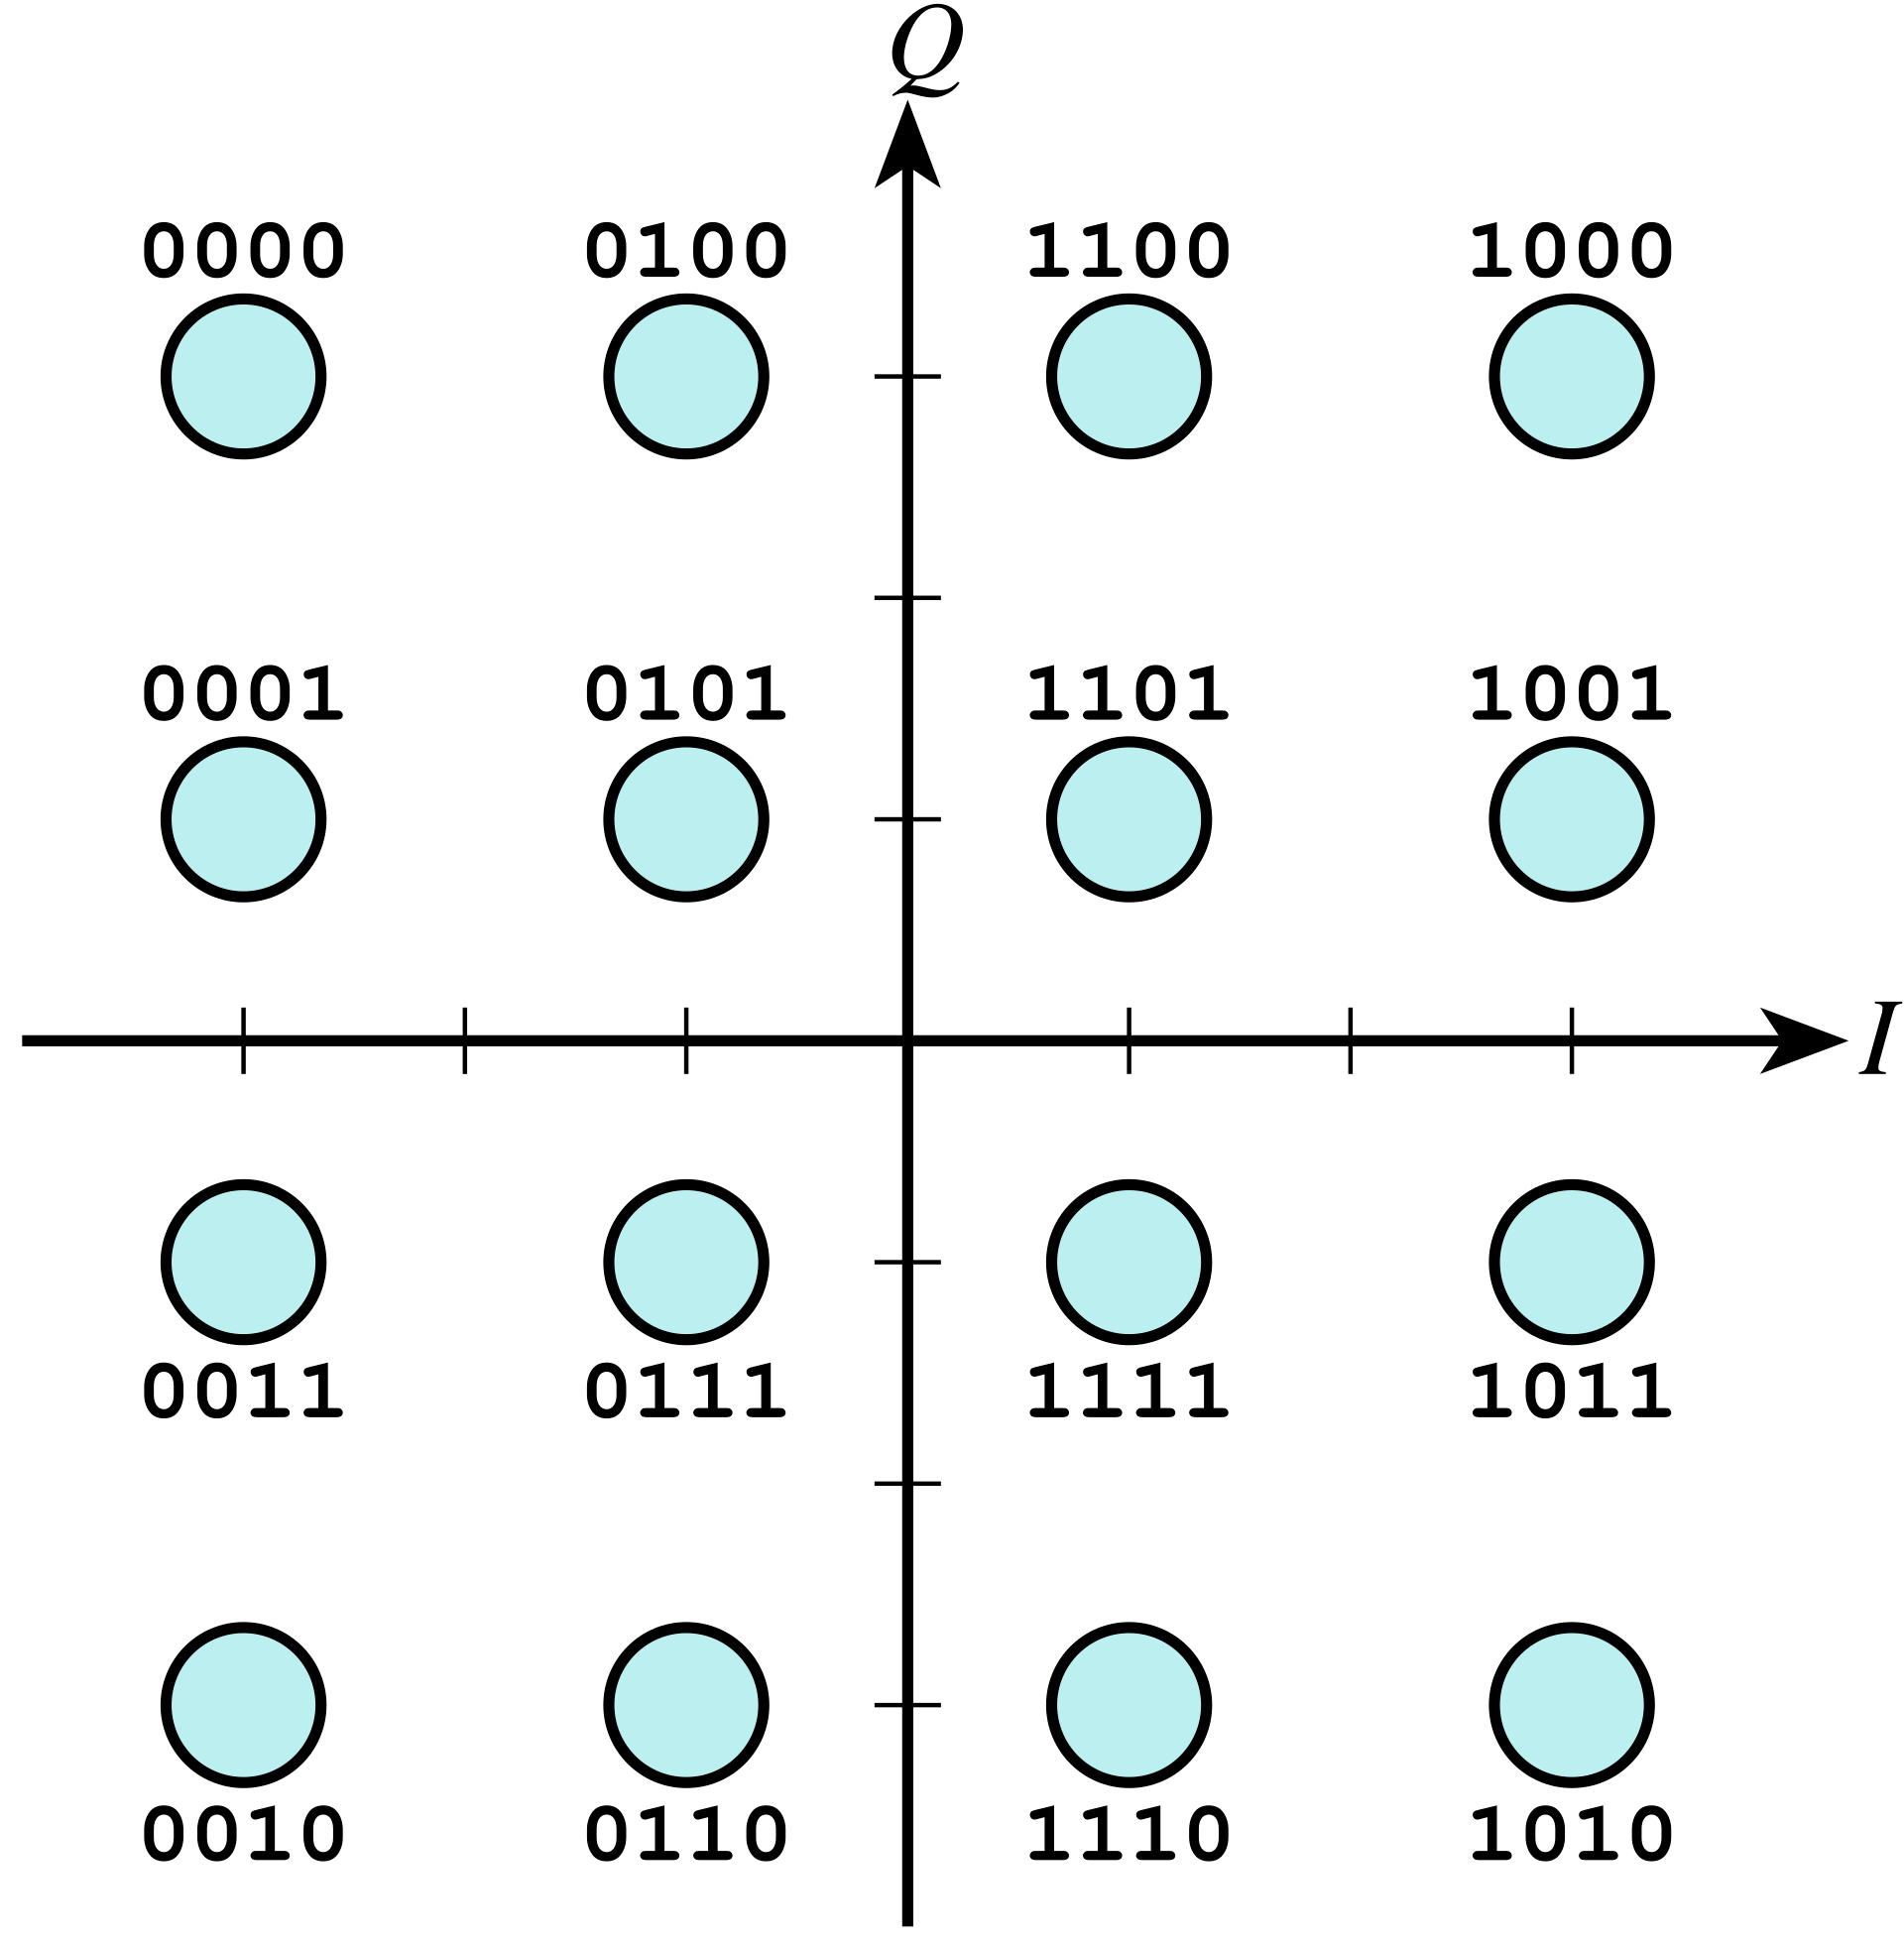
\includegraphics[width=0.5\textwidth]{assets/osi/physical/signals/qam.png}
    \caption{Example of a 16-QAM \textbf{cartesian} constellation diagram}\label{fig:qam_constellation}
\end{figure}


For QAM, the position is determined by the in-phase ($I$) and quadrature ($Q$) components (x, y coordinates). For other modulation schemes:
\begin{itemize}
    \item In PSK, points are arranged in a circle, with phase determining the angular position
    \item In ASK, points are arranged on a line, with amplitude determining the position
\end{itemize}

\begin{importantblock}
    You can probably see that ASK+PSK is QAM, since, by definition, it combines both amplitude and phase modulation.
\end{importantblock}

In any constellation diagram, each point represents a unique combination of signal parameters. The distance between points determines the minimum distance between symbols, which affects the error rate in transmission. The more points we have, the more bits we can transmit per symbol, but the closer they are together, the easier it is to confuse them at the receiver.

There are different ways to visualize these diagrams, for example, when treating ASK+PSK (component-wise, instead as a single complex number), we can plot the amplitude and phase separately as concentric circles with points scattered accross their respective circumferences. This is called a \textbf{polar constellation diagram}.

Let's look at an example of a 4-QAM (ASK+PSK) constellation diagram.
\begin{figure}[h]
    \centering
    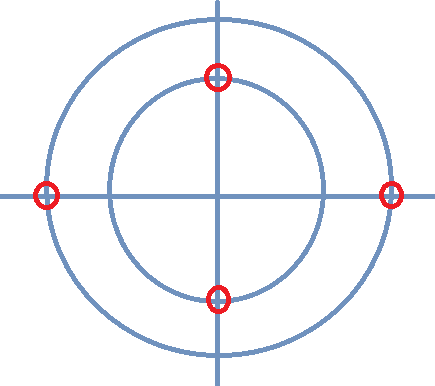
\includegraphics[width=0.5\textwidth]{assets/osi/physical/signals/ask+psk.png}
    \caption{Example of a 4-QAM \textbf{polar constellation diagram}}\label{fig:ask_psk_constellation}
\end{figure}

Now, say we want to encode the binary string \texttt{00101101}. We can map it to the 4-QAM constellation diagram as follows:

\begin{itemize}
    \item \texttt{00} maps to the first point on the left of outer circle
    \item \texttt{10} maps to the second point on the top of inner circle
    \item \texttt{11} maps to the third point on the right of outer circle
    \item \texttt{01} maps to the fourth point on the bottom of inner circle
\end{itemize}

Resulting in the following mapping:
\begin{figure}[h]
    \centering
    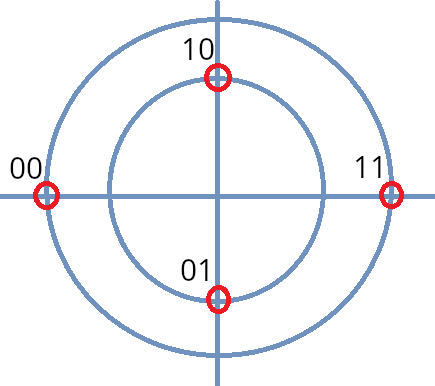
\includegraphics[width=0.5\textwidth]{assets/osi/physical/signals/ask+psk_filled.png}
    \caption{Example of a 4-QAM constellation diagram with bits mapped to points}\
    \label{fig:ask_psk_filled_constellation}
\end{figure}

Again, this mapping is arbitrary, and we can choose any mapping we want, as long as the receiver knows how to interpret it (which, hypothetically, it always does).

Since we have both amplitude and phase information for each constellation point, we can plot the actual time-domain waveforms that correspond to each symbol - showing how the signal actually looks during transmission!

Let's do so for this example.

\subsubsection{Time-Domain Waveforms}
Each constellation point can be expressed as a complex number with amplitude $A$ and phase $\phi$:
$$s(t) = A \cos(2\pi f_c t + \phi)$$

where $f_c$ is the carrier frequency. For our 4-QAM example with bit string \texttt{00101101}, the complete transmitted signal looks like:

\begin{figure}[h]
    \centering
    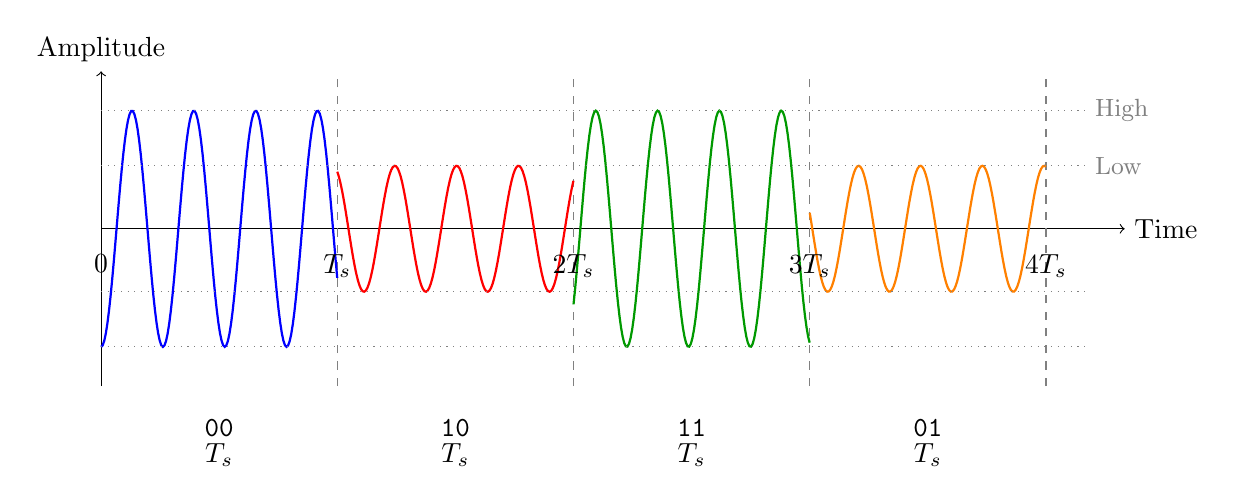
\begin{tikzpicture}[scale=1]
        % Main axes
        \draw[->] (0,0) -- (13,0) node[right] {Time};
        \draw[->] (0,-2) -- (0,2) node[above] {Amplitude};
        
        % Symbol boundaries (vertical dashed lines)
        \foreach \x in {3,6,9,12} {
            \draw[dashed, gray] (\x,-2) -- (\x,2);
        }
        
        % Symbol period labels
        \node[below] at (1.5,-2.3) {\texttt{00}};
        \node[below] at (4.5,-2.3) {\texttt{10}};
        \node[below] at (7.5,-2.3) {\texttt{11}};
        \node[below] at (10.5,-2.3) {\texttt{01}};
        
        % Symbol period markers
        \node[below] at (1.5,-2.6) {$T_s$};
        \node[below] at (4.5,-2.6) {$T_s$};
        \node[below] at (7.5,-2.6) {$T_s$};
        \node[below] at (10.5,-2.6) {$T_s$};
        
        % Complete waveform
        % Symbol 1: 00 (High amp, 180° phase) - inverted high amplitude cosine
        \draw[domain=0:3,samples=150,thick,blue] plot (\x,{1.5*cos(8*\x r + 180)});
        
        % Symbol 2: 10 (Low amp, 90° phase) - low amplitude sine  
        \draw[domain=3:6,samples=150,thick,red] plot (\x,{0.8*cos(8*\x r + 90)});
        
        % Symbol 3: 11 (High amp, 0° phase) - normal high amplitude cosine
        \draw[domain=6:9,samples=150,thick,green!60!black] plot (\x,{1.5*cos(8*\x r)});
        
        % Symbol 4: 01 (Low amp, 270° phase) - low amplitude negative sine
        \draw[domain=9:12,samples=150,thick,orange] plot (\x,{0.8*cos(8*\x r + 270)});
        
        % Amplitude level indicators
        \draw[dotted, gray] (0,1.5) -- (12.5,1.5) node[right] {\small High};
        \draw[dotted, gray] (0,0.8) -- (12.5,0.8) node[right] {\small Low};
        \draw[dotted, gray] (0,-0.8) -- (12.5,-0.8);
        \draw[dotted, gray] (0,-1.5) -- (12.5,-1.5);
        
        % Time axis labels
        \node[below] at (0,-0.2) {0};
        \node[below] at (3,-0.2) {$T_s$};
        \node[below] at (6,-0.2) {$2T_s$};
        \node[below] at (9,-0.2) {$3T_s$};
        \node[below] at (12,-0.2) {$4T_s$};
    \end{tikzpicture}
    \caption{Complete time-domain signal for bit string \texttt{00101101} using 4-QAM modulation. Each symbol period $T_s$ contains one constellation point with its specific amplitude and phase.}
    \label{fig:qam_complete_waveform}
\end{figure}

\begin{tipblock}
    In practice, these individual symbol waveforms are concatenated to form the complete transmitted signal. The receiver uses matched filtering and decision algorithms to determine which constellation point was transmitted by analyzing the received waveform during each symbol period.
\end{tipblock}
% multiplexing
\newpage
\section{Multiplexing}\label{sec:multiplexing}
Okay, we've covered how data gets transmitted over a medium and how we can modulate signals to represent our data. That's cool! Unfortunately, with the busy lives we lead, we need lots of data - fast! So, how do we cram all this data into our limited bandwidth? Enter multiplexing!

Multiplexing is the technique of combining multiple signals into one signal over a shared medium. This allows us to make the most out of our available bandwidth by sending multiple data streams simultaneously. It's exactly like the MUXes you've already seen in Computer Architecture, but now we're applying it to the physical layer of networking.

\subsection{Time Division Multiplexing (TDM)}
\label{subsec:tdm}
Time Division Multiplexing (TDM) shares a single link by slicing time into fixed-length slots. Each source is assigned one slot per frame; sources take turns in a periodic round-robin, so only one transmits at any instant and there is no mutual interference. If a source has nothing to send, its slot may be left idle (synchronous TDM) or reallocated on demand (statistical TDM).

\begin{figure}[h]
    \centering
    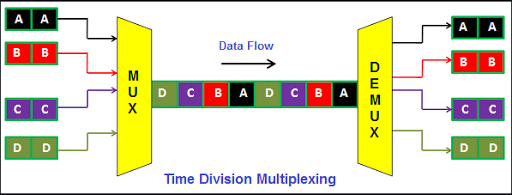
\includegraphics[width=.8\textwidth]{assets/osi/physical/multiplexing/tdm.png}
    \caption{Time Division Multiplexing (TDM) example}
    \label{fig:tdm_example}
\end{figure}

\subsection{Frequency Division Multiplexing (FDM)}
\label{subsec:fdm}
Frequency Division Multiplexing (FDM) is another technique where multiple signals are transmitted simultaneously over different frequency bands. Each signal occupies a unique frequency range, allowing them to coexist without interference. This
is commonly used in radio and television broadcasting, where different channels are assigned specific frequency bands.


TODO


\subsection{Wavelength Division Multiplexing (WDM)}
\label{subsec:wdm}

Wavelength Division Multiplexing (WDM) is a specialized form of FDM used in fiber optic communication. It allows multiple optical signals to be transmitted simultaneously over a single fiber by using different wavelengths (colors) of light. This significantly increases the capacity of the fiber, enabling high-speed data transmission over long distances.


\subsection{Multiple Access}
You might come across the term "multiple access" in networking. Especially in this course. Recall that multiplexing is about sharing a medium among multiple signals (i.e. data streams), which can be thought of as a single device (or two, in the case of communication), sending multiple signals at once towards each other.

\begin{importantblock}
    Multiple access, on the other hand, is about how \textbf{multiple devices} share a medium to communicate with each other.
\end{importantblock}

\subsection{Code Division Multiple Access (CDMA)}
\label{subsec:cdma}
Code Division Multiple Access (CDMA) allows multiple signals to share the same frequency band simultaneously. Unlike TDMA or FDMA, CDMA uses unique code sequences called "chip codes" to distinguish between different users' signals.

\paragraph{How Chip Codes Work}


Each transmitter receives a unique binary sequence (chip code) with these properties:
\begin{itemize}
    \item Much longer than data bits (typically 64-128 chips per bit)
    \item Mathematically orthogonal to other users' codes
    \item Produces strong correlation when multiplied by itself
    \item Produces near-zero correlation with different codes
\end{itemize}

When sending data, each bit is multiplied by the entire chip code. The receiver recovers the original data by multiplying the received signal with the same code and integrating over the bit period.


\begin{figure}[h]
    \centering
    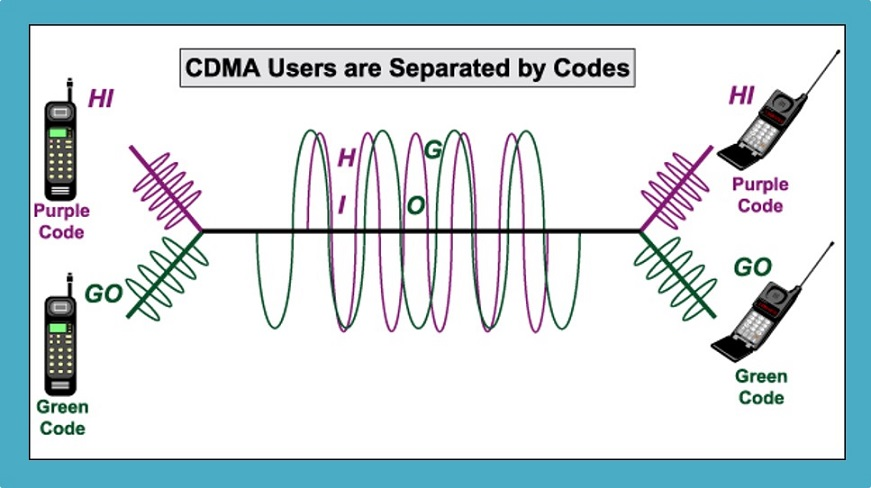
\includegraphics[width=0.7\textwidth]{assets/osi/physical/multiplexing/cdma_example.png}
    \caption{CDMA encoding showing how data bits are spread using chip codes}
    \label{fig:cdma_example}
\end{figure}


\subsubsection{Orthogonality of Chip Codes $\star$}

CDMA deals with the problem of multiple users transmitting simultaneously. We can make the analogy with multiple people talking over each other: if everyone speaks over each other, it's a mess. But if the group involved is comprise of pairs of people, each speaking their own, completely different language, they can communicate without interference (because they can't understand anyone but their partner). 

The "languages" in CDMA are called \textbf{chip codes} - patterns that are mathematically orthogonal to each other. Orthogonality, in math terms, means that two vectors are perpendicular to each other, so they don't interfere with each other when projected onto a common space.

In everyday life, orthogonality appears in many forms. Think of noise-canceling headphones: they work by generating sound waves that are "orthogonal" (phase-inverted) to ambient noise, effectively canceling it out. Similarly, polarized sunglasses use orthogonal light wave orientations to block glare - light waves vibrating in one direction are blocked while those in the perpendicular direction pass through.

\begin{importantblock}
    Two codes are orthogonal when their dot product equals zero. This means they don't interfere with each other, allowing perfect separation at the receiver.
\end{importantblock}

Let's take a look at how this works in practice. We have two users, each with their own chip codes:
\begin{align*}
\vec{c_1} &= [1, -1, 1, -1]\\
\vec{c_2} &= [1, 1, -1, -1]
\end{align*}
And data:
\begin{align*}
d_1 &= [1, 0, 1, 0]\\
d_2 &= [0, 1, 0, 1]
\end{align*}

Verifying orthogonality of chip codes (just to drive the point home, you don't need to do this in practice):
\begin{align*}
\vec{c_1} \cdot \vec{c_2} &= (1)(1) + (-1)(1) + (1)(-1) + (-1)(-1)\\
&= 1 - 1 - 1 + 1 = 0
\end{align*}

\subsubsection{Encoding Data}


When encoding, each data bit controls the direction of the chip code vector:
\begin{itemize}
    \item For a bit value of 1: Use the original chip code
    \item For a bit value of 0: Use the inverted chip code (multiply by -1)
\end{itemize}

Because the chip codes are orthogonal to each other, the receiver can extract each user's data by projecting the combined signal onto their respective code direction, effectively filtering out other users' data.

So, for our running example, we have:

User 1:
\begin{align*}
d_1[0]=1: \underbrace{[1, -1, 1, -1]}_{\text{chip code for bit 1}}\\
d_1[1]=0: \underbrace{[-1, 1, -1, 1]}_{\text{chip code for bit 0}}\\
d_1[2]=1: \underbrace{[1, -1, 1, -1]}_{\text{chip code for bit 1}}\\
d_1[3]=0: \underbrace{[-1, 1, -1, 1]}_{\text{chip code for bit 0}}\\
\end{align*}
So for user 1, the encoded signal is:
\begin{align*}
\vec{s_1} &= [1, -1, 1, -1, -1, 1, -1, 1, 1, -1, 1, -1, -1, 1, -1, 1]
\end{align*}

For user 2, skipping the details, we get:
\begin{align*}
\vec{s_2} &= [-1, -1, 1, 1, 1, 1, -1, -1, -1, -1, 1, 1, 1, 1, -1, -1]
\end{align*}

Finally, the combined (transmitted) signal is:
\begin{align*}
\vec{s} &= \vec{s_1} + \vec{s_2} = [0, -2, 2, 0, 0, 2, 0, 0, 0, -2, 2, 0, 0, 2, 0, 0]
\end{align*}

\subsubsection{Decoding Data}
To decode, the receiver multiplies the received signal by each chip code and integrates over the bit period. In other words, we compute the dot product of the received signal with each chip code, generally like this:

\[
d_i = \frac{\vec{s} \cdot \vec{c_i}}{|\vec{c_i}|^2}
\quad\text{ or }\quad
d_i = \frac{\vec{s} \cdot \vec{c_i}}{\sum_{j=1}^{n} c_{i,j}^2}
\quad\text{ or even }\quad
d_i = \frac{\sum{s_j c_{i,j}}}{\sum_{j=1}^{n} c_{i,j}^2}
\]

Where $d_i$ is the decoded data for user $i$, $\vec{s}$ is the received signal, and $\vec{c_i}$ is the chip code for user $i$. The denominator normalizes the result based on the length of the chip code. Try to understand why this works: it essentially projects the received signal onto the chip code vector, giving us the original data bit.

In pure English, the process works as follows:
\begin{enumerate}
    \item Take the received combined signal for one bit period
    \item Project it onto each user's chip code direction (dot product)
    \item The projection magnitude tells us the bit value:
    \begin{itemize}
        \item Positive projection → bit = 1
        \item Negative projection → bit = 0
        \item Zero projection → no signal from this user
    \end{itemize}
\end{enumerate}

For user 1, decoding the first bit:
For user 1, decoding the first bit:
\begin{align*}
d_{1,0} &= \frac{\sum_{j=0}^{3} s_j c_{1,j}}{\sum_{j=0}^{3} c_{1,j}^2}\\
&= \frac{(0)(1) + (-2)(-1) + (2)(1) + (0)(-1)}{(1)^2 + (-1)^2 + (1)^2 + (-1)^2}\\
&= \frac{0 + 2 + 2 + 0}{1 + 1 + 1 + 1}\\
&= \frac{4}{4} = 1
\end{align*}

Similarly, for all bits and users:

User 1:
\begin{align*}
d_{1,0} &= \frac{\sum_{j=0}^{3} s_j c_{1,j}}{\sum_{j=0}^{3} c_{1,j}^2} = \frac{4}{4} = 1 \\
d_{1,1} &= \frac{\sum_{j=4}^{7} s_j c_{1,j}}{\sum_{j=0}^{3} c_{1,j}^2} = \frac{-4}{4} = -1 \approx 0 \\
d_{1,2} &= \frac{\sum_{j=8}^{11} s_j c_{1,j}}{\sum_{j=0}^{3} c_{1,j}^2} = \frac{4}{4} = 1 \\
d_{1,3} &= \frac{\sum_{j=12}^{15} s_j c_{1,j}}{\sum_{j=0}^{3} c_{1,j}^2} = \frac{-4}{4} = -1 \approx 0
\end{align*}

User 2:
\begin{align*}
d_{2,0} &= \frac{\sum_{j=0}^{3} s_j c_{2,j}}{\sum_{j=0}^{3} c_{2,j}^2} = \frac{-4}{4} = -1 \approx 0 \\
d_{2,1} &= \frac{\sum_{j=4}^{7} s_j c_{2,j}}{\sum_{j=0}^{3} c_{2,j}^2} = \frac{4}{4} = 1 \\
d_{2,2} &= \frac{\sum_{j=8}^{11} s_j c_{2,j}}{\sum_{j=0}^{3} c_{2,j}^2} = \frac{-4}{4} = -1 \approx 0 \\
d_{2,3} &= \frac{\sum_{j=12}^{15} s_j c_{2,j}}{\sum_{j=0}^{3} c_{2,j}^2} = \frac{4}{4} = 1
\end{align*}

So we've successfully recovered our original data: $d_1 = [1, 0, 1, 0]$ and $d_2 = [0, 1, 0, 1]$.

\newpage
\subsection{TDMA and FDMA}
\label{subsec:tdma_fdma}

Now that we've seen how CDMA works, let's look at two other fundamental multiple access techniques: TDMA and FDMA. These approaches solve the same problem (multiple users sharing a medium) but use completely different strategies.

\subsubsection{TDMA}
Think of TDMA like a well-organized conversation. Everyone gets to speak, but they take turns - only one person talks at a time, and everyone else listens. When your turn comes, you have the floor completely to yourself.

This approach to resource allocation is called \textbf{round-robin} schedule: users take turns in a fixed order, each occupying one time slot per frame; after the last user, the sequence repeats.

\begin{figure}[h]
    \centering
    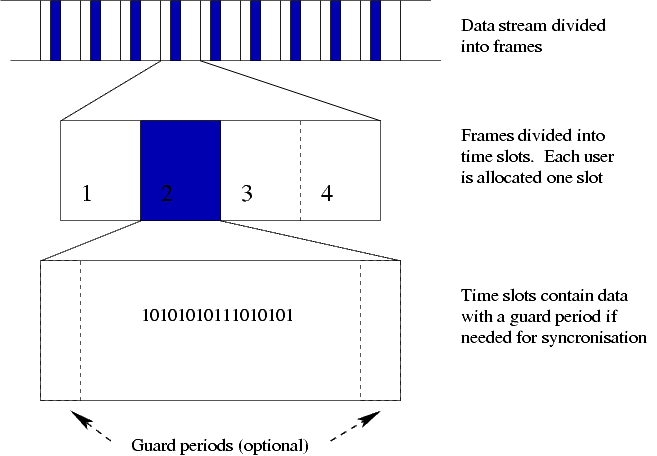
\includegraphics[width=0.8\textwidth]{assets/osi/physical/multiplexing/tdma.png}
    \caption{TDMA: Users take turns transmitting in fixed time slots}
    \label{fig:tdma}
\end{figure}

In TDMA:
\begin{itemize}
    \item The entire frequency band is available to each user
    \item Time is divided into fixed slots (called a "frame")
    \item Each user gets one slot per frame
    \item Users transmit in round-robin fashion
    \item If a user has nothing to send, their slot remains empty
\end{itemize}


\subsubsection{FDMA}
FDMA has multiple dedicated perceptual "lanes" that users can occupy called channels. This is like FM radio, WiFi or even cable TV, where each channel is a separate frequency band.

\begin{figure}[h]
    \centering
    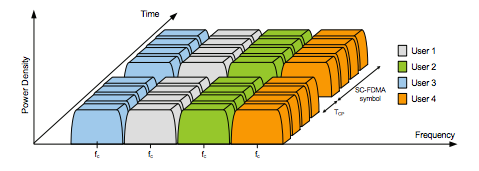
\includegraphics[width=0.8\textwidth]{assets/osi/physical/multiplexing/fdma-sc.png}
    \caption{FDMA: Users transmit simultaneously on different frequency bands}
    \label{fig:fdma}
\end{figure}

In FDMA:
\begin{itemize}
    \item Each user gets a dedicated frequency band (channel)
    \item All users can transmit simultaneously
    \item Guard bands separate channels to prevent interference
    \item Users can transmit whenever they want within their assigned frequency
\end{itemize}

Modern systems often combine these techniques! For example:
\begin{itemize}
    \item \textbf{4G LTE}: Uses both FDMA (different frequency carriers) and TDMA (time slots within each carrier)
    \item \textbf{Wi-Fi}: Uses FDMA (different channels) plus collision avoidance protocols
    \item \textbf{GPS}: Uses CDMA for satellites plus FDMA for different frequency bands
\end{itemize}

\begin{importantblock}
    Remember: These are all solutions to the same fundamental problem - how do multiple users share a limited communication medium without interfering with each other? The "best" solution depends on your specific requirements for capacity, latency, complexity, and cost.
\end{importantblock}

\subsection{Carriers and Sensing}
\label{subsec:carriers_sensing}
As you might have noticed in Figure \ref{fig:fdma}, the graph is labelled as FDMA-SC, where the SC stands for \textbf{Single Carrier}. But what is a carrier? We've also seen that word in Section \ref{sec:modulation} when we talked about modulating signals.

\begin{importantblock}
    A carrier is a signal that can be modulated to carry information. Usually a sine wave, we augment it by modulating its amplitude, frequency, or phase to encode our data (as we mentioned in Section \ref{sec:modulation}).
\end{importantblock}

Sensing is the process of detecting whether a signal is already present on a carrier frequency. This allows devices to determine if a channel is busy or available before attempting to transmit. In TDMA systems, sensing helps verify if it's the designated time slot for transmission. In FDMA systems, sensing checks whether the assigned frequency band is clear of interference.

This brings us to a perfect (in the author's opinion) segue: carrier sensing addresses collision detection, but collision handling and recovery falls under the Data Link Layer of the OSI model. You're in luck! Enter\dots

